\documentclass[10pt,twocolumn]{article}

\usepackage[letterpaper,top=0.75in,bottom=0.75in,left=0.7in,right=0.7in,columnsep=0.28in]{geometry}
\usepackage{graphicx}
\usepackage{booktabs}
\usepackage{xcolor}
\usepackage{hyperref}
\usepackage{enumitem}
\usepackage{caption}
\setlength{\parindent}{0pt}
\setlength{\parskip}{4pt plus 1pt minus 1pt}
\setlength{\emergencystretch}{3em}  % absorb long monospace words in narrow columns

\hypersetup{
  colorlinks=true,
  linkcolor=teal!60!black,
  citecolor=teal!60!black,
  urlcolor=teal!60!black,
}

\definecolor{accent}{HTML}{2A4A7F}
\definecolor{supervisor}{HTML}{C4632C}
\definecolor{blackboard}{HTML}{2C8485}
\definecolor{mcts}{HTML}{6A4F8A}
\definecolor{ok}{HTML}{2F7A3D}
\definecolor{bad}{HTML}{A8302C}

\captionsetup{font=small, labelfont=bf, labelsep=period}

\title{\textbf{Speculative Context: A Pool-Based Cache for\\ SOP-Constrained Voice Agents}}
\author{Dima (Dan) Sivov\\ \texttt{dsivov@gmail.com}}
\date{June 2026}

\begin{document}

\twocolumn[{%
  \centering
  {\LARGE\bfseries Speculative Context: A Pool-Based Cache for SOP-Constrained Voice Agents\par}
  \vspace{10pt}
  {\large Dima (Dan) Sivov\par}
  {\normalsize\texttt{dsivov@gmail.com}\par}
  \vspace{4pt}
  {\normalsize June 2026\par}
  \vspace{14pt}
  \begin{minipage}{0.86\textwidth}
    \small
    \textbf{Abstract.} Real-time voice agents face a latency--intelligence trade-off: a small fast model holds the conversational budget but cannot reason through multi-step procedures or retrieve documents, while a large model can but leaves the user waiting---above all on slow external data. We present a two-system architecture for voice agents under a declared Standard Operating Procedure (SOP): a live agent reads from a session-scoped knowledge \emph{pool} that an off-path \emph{supervisor} populates speculatively during the user's speech-time, moving external-data retrieval off the critical path. We evaluate three components. (i)~A \textbf{speculatively-populated pool cache}: because mispredicted fetches remain usable pool candidates rather than discarded cache misses, per-turn curation supplies a prefetched item on 96\% of turns, whereas an exact-key cache consumes only 11\% of the same speculative fetches (two distinct metrics; \S\ref{sec:pool}); across our sessions this hides a mean of 22.5\,s of external-data latency per conversation. (ii)~A \textbf{cosine-plus-dedup rerank} that curates the pool with no LLM on the critical path; on a matched comparison it reproduces an LLM reranker's curation while cutting p95 rerank latency from 2167\,ms to 940\,ms (299\,ms mean / 483\,ms p95 in the locked cross-SOP configuration). (iii)~A \textbf{speculative-context prompt}: an ablation shows that labelling prefetched items honestly as speculative---rather than ``curated, high-relevance''---keeps the agent from over-using low-relevance items on conversation-closing turns. We are explicit about scope ($N{=}5$ per cell, simulator users, internal baselines) and report the end-to-end picture: the rerank adds only $\sim$300\,ms, while total turn time ($\sim$6\,s) is dominated by the live agent's own two LLM calls---which a smaller model does not reduce (\S\ref{sec:e2e})---so this work targets external-data latency, not LLM-inference latency.
  \end{minipage}
  \vspace{18pt}
}]

%======================================================================
\section{Introduction}
%======================================================================

A real-time voice agent makes a choice on every turn that has no good answer under a single model. A small fast model holds the real-time budget but fumbles whenever it must follow a multi-step procedure or retrieve a document; a large model is competent but leaves five to fifteen seconds of silence between utterances, and users hang up. The standard production compromise---a medium model with a thin retrieval layer and a router that escalates hard cases---works for simple flows but not for the regulated, multi-step conversations (insurance renewal, medical scheduling, account servicing) that businesses actually need handled.

We treat the trade-off as a \emph{two-system} problem rather than a one-model problem. A fast live agent responds in real time, reading from a shared blackboard. A slow supervisor runs in the background between user utterances---during the user's own speech-time---predicting what the user will need next and pre-staging it. When the supervisor is right, the response feels instant; when wrong, the live agent falls back to its built-in behaviour, no worse than today. Framed quantitatively, the supervisor solves a budgeted prediction problem: choose, within a fixed speculative-compute budget, which upcoming data dependencies to prefetch so as to minimise the critical-path latency the live agent pays---the \emph{regret} against a perfect-foresight oracle (\S\ref{sec:related}). The general orientation (use the user's speech-time for slow work) appears in AsyncMLD~\cite{asyncmld2023} for dialogue recommendation; our contribution is the specific design that makes it work for SOP-constrained voice dialogue.

\textbf{Contributions.}
\begin{enumerate}[leftmargin=*, itemsep=3pt]
\item A \textbf{speculatively-populated pool cache} (\S\ref{sec:pool}). Rather than predict an exact cache key, the supervisor appends each speculatively-fetched item to a session-scoped pool; the live agent curates it per turn. Because mispredictions persist as pool candidates instead of being discarded, per-turn curation supplies a prefetched item on 96\% of turns, whereas an exact-key cache over the same speculative fetches consumes only 11\% of them (two different denominators, reconciled in \S\ref{sec:pool}). The novel element is the misprediction-tolerant \emph{population} policy over an SOP graph, not the dual-agent prefetch-cache pattern itself (\S\ref{sec:related}).
\item \textbf{An empirical case that the per-turn rerank needs no LLM} (\S\ref{sec:rerank-design}, \S\ref{sec:abl-rerank}). Our curation is cosine ranking plus a thresholded redundancy filter (a form of MMR~\cite{mmr1998}); the contribution is the measurement that this recovers an LLM reranker's \emph{only} value-add on this data---near-duplicate avoidance---while removing it from the critical path. On a matched comparison this cuts p95 rerank latency from 2167\,ms to 940\,ms with no loss of curation quality.
\item \textbf{A framing-mismatch ablation for speculative context} (\S\ref{sec:prompt-design}, \S\ref{sec:abl-prompt}). That LLMs degrade on irrelevant context and that an ``ignore irrelevant information'' instruction mitigates it is known~\cite{shi2023}; what we add is an ablation in an asynchronous prefetch pipeline showing that an over-confident ``curated'' label (vs.\ an honest ``speculative'' one) makes the agent over-use low-relevance items on conversation-closing turns, lowering task success.
\end{enumerate}

We evaluate on two SOPs (outbound car-insurance renewal, inbound medical-appointment booking) using a smart-LLM customer simulator. The present study is deliberately scoped---$N{=}5$ per cell, simulator users, internal baselines---and \S\ref{sec:limitations} states the controlled experiments (larger $N$ with confidence intervals, published-baseline comparisons, a human study via a live-avatar harness we have built) that complete it.

%======================================================================
\section{Related work}
\label{sec:related}
%======================================================================

\textbf{Voice agents with speech-time speculative prefetch (closest work).} The dual-agent shape we adopt---a background agent that prefetches during the user's speech and a foreground agent that reads from the resulting cache---has been explored concurrently in real-time voice systems. Closest is VoiceAgentRAG~\cite{voiceagentrag2026}, whose background ``Slow Thinker'' predicts likely follow-up topics with an LLM and prefetches document chunks into a semantic cache that a foreground ``Fast Talker'' reads on cache hits; LTS-VoiceAgent~\cite{lts2026} (``listen--think--speak'') and RelayS2S~\cite{relays2s2026} similarly overlap background reasoning with foreground speech, and predictive-ASR prefetch~\cite{predasr2023} hides downstream latency by acting on a preliminary ASR hypothesis. We do not claim the dual-agent speech-time-prefetch pattern itself as novel. We differ in two respects that we evaluate: (i) our supervisor predicts over a \emph{structured SOP graph} using empirical transition statistics (with optional MCTS lookahead), rather than free-form topic prediction; and (ii) our pool is \emph{misprediction-tolerant}---a fetch triggered by a wrong prediction remains a curated candidate on later turns instead of becoming a wasted cache entry (\S\ref{sec:pool}).

\textbf{Asynchronous LLM work during dialogue.} AsyncMLD~\cite{asyncmld2023} reduces dialogue-system latency by running database searches and intention understanding in parallel with the agent's spoken response. We share the orientation---do slow work during the user's speech-time---but differ in mechanism: rather than dispatching parallel work for the \emph{current} query, our supervisor maintains a session-scoped pool of speculatively prefetched items, curated per turn for the \emph{next} response.

\textbf{Planning-based dialogue and speculative tool execution.} ChatSOP~\cite{chatsop2024} introduces Monte Carlo Tree Search (MCTS) over an SOP graph for controllable LLM dialogue. Our supervisor's planner is of this family; the architectural delta is that planning runs off the critical path, contributing predictions to the pool rather than gating the live reply. Most directly related to our prefetch mechanism is PASTE~\cite{paste2026}, which speculatively pre-executes tools during an agent's reasoning time using patterns mined from execution traces---and finds, as we do, that trace-mined prediction outperforms search-based lookahead for deciding what to fetch; our ablation (\S\ref{sec:abl-predictor}) reaches the same conclusion against MCTS for dialogue data prefetch. We differ in slack window (the user's speech-time vs.\ the LLM's reasoning-time) and in misprediction handling: PASTE discards mispredictions on a bounded budget, whereas our pool \emph{retains} them as reusable candidates.

\textbf{Bandits, regret, and budgeted prefetch.} Choosing \emph{which} upcoming data dependencies to prefetch under a fixed speculative budget is a budgeted, contextual multi-armed bandit~\cite{lairobbins1985,auer2002,licontextual2010,bwk2018}: each candidate dependency is an arm with uncertain payoff (latency saved on a pool hit), the budget caps the pulls per turn, the context is (cohort, state, mood, history), and the objective is to minimise \emph{regret}---the latency a perfect-foresight oracle would have saved but we did not (see~\cite{slivkins2019} for a survey). Our system occupies the exploit-only corner of this space: the empirical predictor prefetches the historically best-paying arms and never explores, which \S\ref{sec:abl-predictor} justifies for a near-stationary SOP policy that counting estimates well. We also evaluate a frozen predictor, so our 4.5\% (\S\ref{sec:cross-sop}) is a converged point estimate, not cumulative learning regret. Online exploration---warranted at cold start and under non-stationarity---is the bandit generalisation we leave to future work (\S\ref{sec:limitations}).

\textbf{Caching and reranking.} Similarity-based caches such as GPTCache~\cite{gptcache2023} rescue near-miss lookups that exact-key caches discard---the premise our pool builds on, but applied to \emph{speculatively prefetched data} rather than reactively cached responses. Cache-augmented generation~\cite{cag2024} and session-scoped vector retrieval reuse accumulated context without re-paying per turn; agentic plan caching~\cite{plancache2025} reuses cached \emph{plans} across similar tasks (we reuse prefetched \emph{data}). Our per-turn curation is deliberately lightweight: the dedup step---cosine ranking plus cosine-threshold redundancy removal---is a thresholded form of Maximal Marginal Relevance~\cite{mmr1998}, and the empirical contribution of \S\ref{sec:abl-rerank} is the measurement that this recovers an LLM reranker's only value-add (near-duplicate avoidance) at a fraction of its latency. Speculative decoding~\cite{speculativedecoding2023} bets on a likely future at the token level and falls back when wrong; our ``speculative'' is at the data/context layer, but the speculate-then-verify heritage is the same. We also distinguish our usage from Speculative RAG~\cite{specrag2024}, where ``speculative'' denotes small-model \emph{draft}-and-verify at answer time; ours denotes \emph{prefetch} during the user's speech-time, a different mechanism and layer.

\textbf{Irrelevant-context robustness.} That LLMs degrade on irrelevant context---and that a simple instruction to ignore it mitigates the effect---was shown by Shi et al.~\cite{shi2023}. Our speculative-context prompt (\S\ref{sec:abl-prompt}) applies this in an asynchronous prefetch pipeline; what we add is the \emph{framing-mismatch} ablation (an over-confident ``curated'' label vs.\ an honest ``speculative'' one) and the closing-turn failure mode it exposes.

%======================================================================
\section{Architecture}
\label{sec:arch}
%======================================================================

\begin{figure*}[t]
\centering
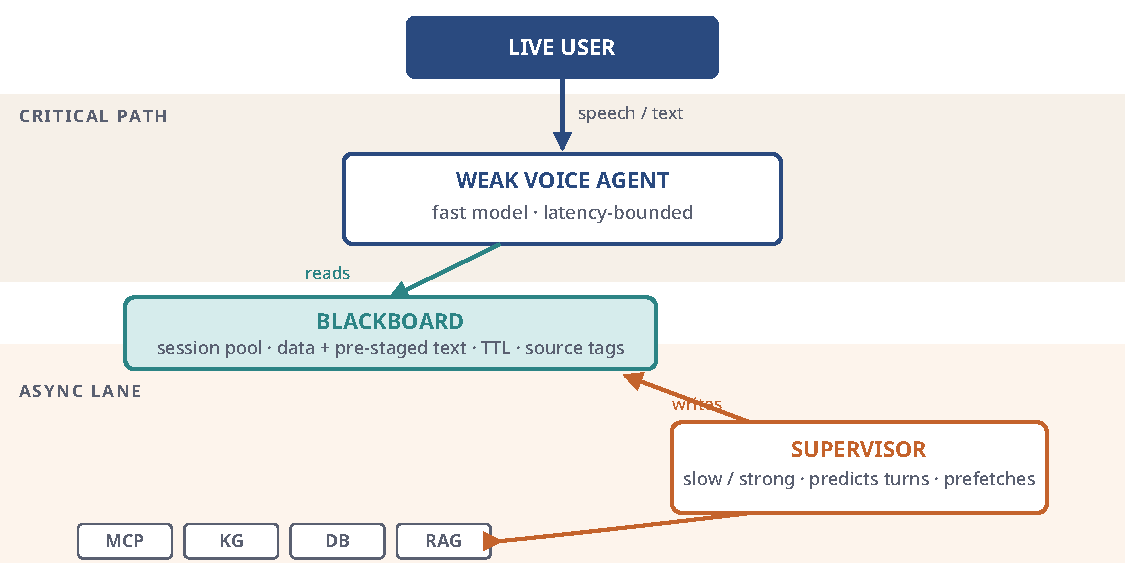
\includegraphics[width=0.78\linewidth]{figs/fig1_two_system.pdf}
\caption{The two-system architecture. The live voice agent talks only to the shared blackboard, never to the supervisor or data sources directly. The supervisor runs slow work (search, retrieval, planning) during the gap between user utterances and writes results to the blackboard.}
\label{fig:two-system}
\end{figure*}

The live voice agent (\texttt{gpt-4o} in our implementation) reads the shared blackboard---a per-session pool of prefetched items, each tagged with provenance and a TTL. In the common case it does not block on external I/O, serving data dependencies from the pool; it falls back to a blocking live fetch only on the rare turn where a needed dependency was not prefetched (9 such fetches in the runs of \S\ref{sec:cross-sop}). All other slow work---retrieval, planning, reasoning over the conversation graph---is done off-path by the supervisor (Figure~\ref{fig:two-system}).

\subsection{SOP structure}

The conversation is structured by a declared SOP: a directed graph whose nodes are \emph{agent actions} (e.g.\ \texttt{VerifyIdentity}, \texttt{PitchDiscount}) and \emph{user states} (e.g.\ \texttt{PriceConcern}, \texttt{AgreedToRenew}), with edges encoding allowed transitions. Each agent action declares its external \emph{data dependencies} (a policy lookup, a market-rates query, a discounts retrieval). Cohorts and per-cohort moods describe the user's archetype and disposition and shape both the supervisor's predictions and the live agent's style (Figure~\ref{fig:sop-graph}). The supervisor plans against this graph: from the current state it predicts the next 1--3 likely user states, the agent actions that would follow, and prefetches those actions' data dependencies.

\begin{figure*}[t]
\centering
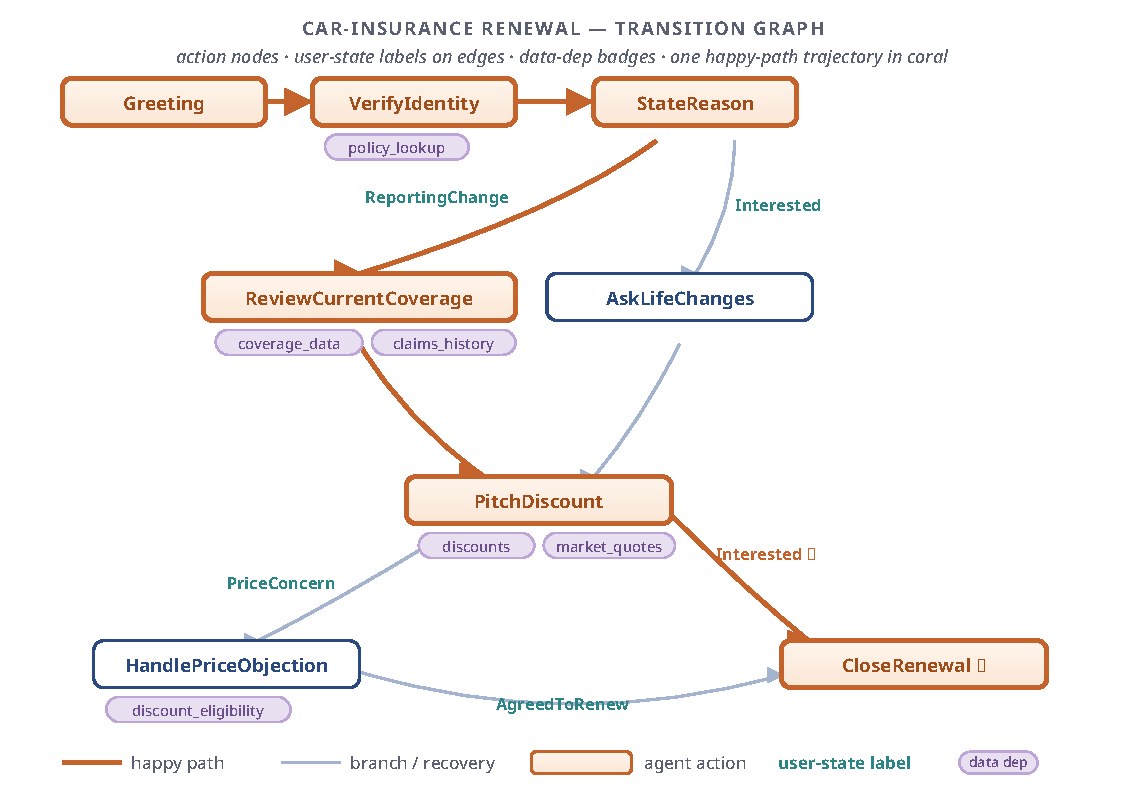
\includegraphics[width=0.82\linewidth]{figs/fig4_sop_transition_graph.pdf}
\caption{The car-insurance renewal SOP, with a representative happy-path trajectory (coral) and off-trajectory recovery branches (grey). User-state labels sit on edges; data-dependency badges sit under the action that prefetches them. The full SOP has 13 actions, 11 user states, and 7 cohorts $\times$ 3--4 moods.}
\label{fig:sop-graph}
\end{figure*}

\subsection{The supervisor's predictor stack}

Two predictors populate the pool, plus a fallback. An \textbf{empirical predictor} (the workhorse) looks up accumulated \texttt{precedent\_traces} for the action distribution that historically follows the current (cohort, state, action), and schedules prefetches for those actions' dependencies; it is cheap, deterministic, and improves as deployment data accumulates. \textbf{Background MCTS pondering} (\S\ref{sec:pondering}) is a more far-sighted predictor: it runs speculative tree search over the SOP during the user's speech-time. We retain it in the architecture but show by ablation (\S\ref{sec:abl-predictor}) that it does not earn its cost on the retrieval task; the generative part of retrieval is instead supplied by a single cheap LLM call (\S\ref{sec:abl-predictor}). Distinct from these is a \textbf{blocking live fallback}: when a needed dependency was \emph{not} prefetched, the live agent issues it synchronously on the critical path (these are misses, not predictions, counted separately in \S\ref{sec:cross-sop}). In our measured configuration the empirical predictor supplies the large majority of pool items.

\subsection{Background MCTS pondering}
\label{sec:pondering}

Between turns the supervisor does not yet know what the user will say---but the SOP sharply constrains the possibilities. The next user state is drawn from a small vocabulary, and the empirical transition statistics make some states far more likely than others. Pondering exploits this idle window. When a turn ends, the supervisor (i)~predicts the top-$K$ most likely next user states from the empirical transition frequencies over accumulated precedent traces, and (ii)~spawns one Monte Carlo Tree Search per hypothesized state, all running in the background while the user is still speaking (Figure~\ref{fig:pondering}). None of this is on the critical path; if the next turn arrives first, the searches are simply cancelled.

\begin{figure*}[t]
\centering
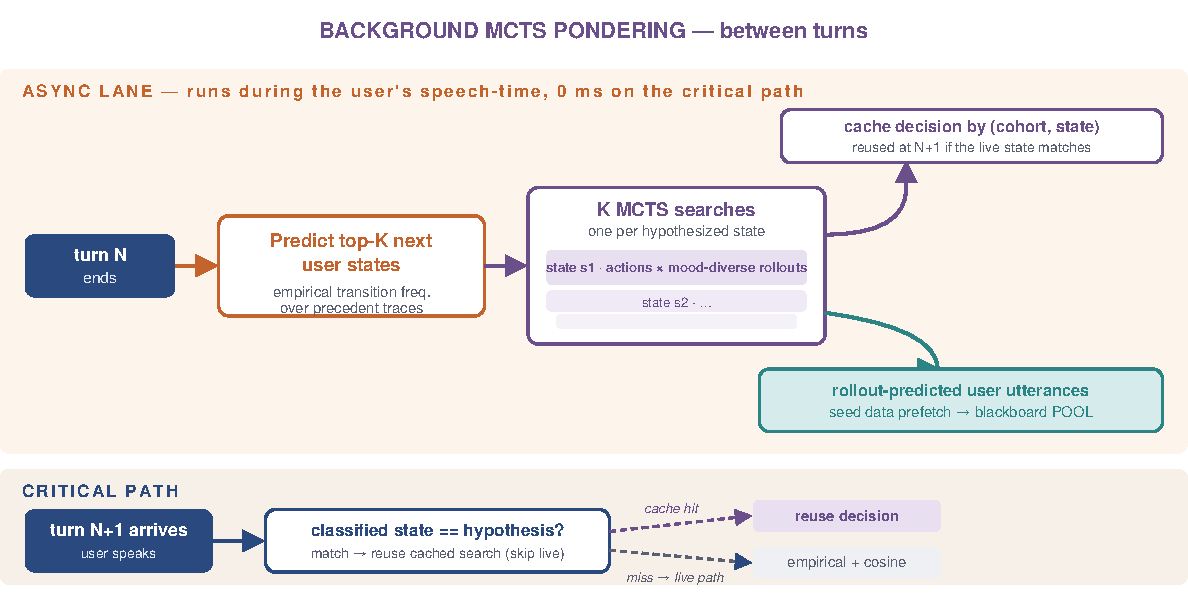
\includegraphics[width=0.82\linewidth]{figs/fig7_pondering_flow.pdf}
\caption{Background MCTS pondering. When turn $N$ ends, the supervisor predicts the top-$K$ likely next user states and runs one MCTS search per state during the user's speech-time. The searches yield two payoffs: a cached action decision (reused at turn $N{+}1$ if the live state matches a hypothesis) and rollout-predicted user utterances that seed data prefetch into the pool. Everything happens off the critical path.}
\label{fig:pondering}
\end{figure*}

Each search is an MCTS over the SOP action graph (depth~3 in our configuration), with one twist that matters for prefetch diversity: rollouts are \emph{mood-diverse}. Each cohort carries a small vocabulary of moods---dispositions such as \texttt{price\_anxious} or \texttt{calm\_negotiator}---with prior probabilities. At the start of each rollout the simulated user's mood is sampled from that prior and held fixed for the rollout. Parallel rollouts under the same candidate action therefore explore genuinely different user dispositions, which react differently to the same agent move, and the action's value is the reward averaged across those mood draws (Figure~\ref{fig:rollout}). Without mood diversity, rollouts collapse onto a single ``average'' user and the predicted next-state distribution is artificially narrow; mood sampling widens it, which in turn diversifies what the supervisor prefetches.

\begin{figure*}[t]
\centering
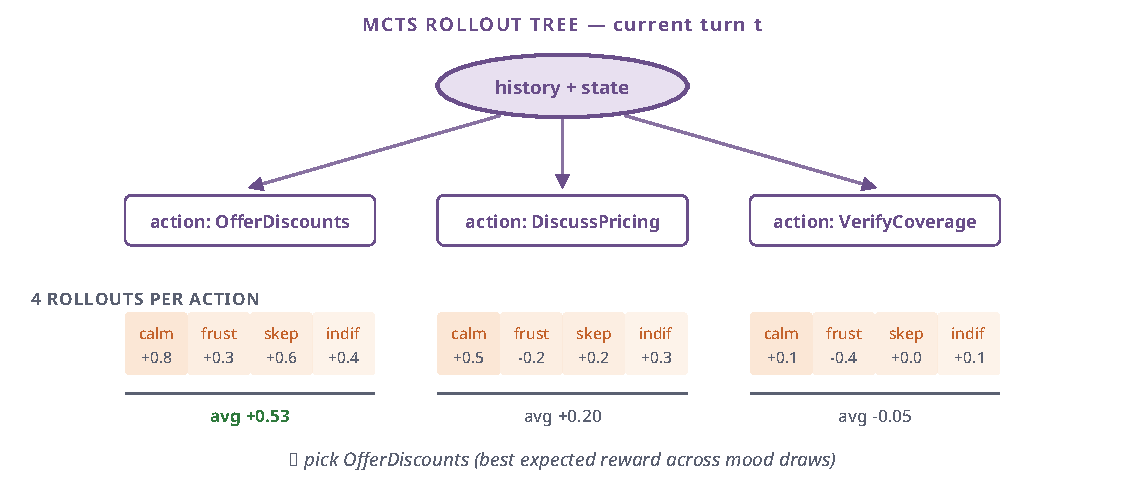
\includegraphics[width=0.74\linewidth]{figs/fig2_mcts_rollout_tree.pdf}
\caption{One pondering search for a single hypothesized next state. Candidate agent actions (here three) are each evaluated by mood-diverse rollouts---a draw per cohort mood (calm, frustrated, skeptical, indifferent)---and the action's value is the mean reward across mood draws. The best action is cached for reuse if this hypothesized state is the one the user actually reaches.}
\label{fig:rollout}
\end{figure*}

A completed pondering search yields two payoffs, both feeding the live turn that follows. First, a \textbf{cached action decision}, keyed by (cohort, predicted state): if the user's actual classified state at turn $N{+}1$ matches a hypothesis, the live agent reuses the cached search and skips live planning entirely. Second, \textbf{prefetch seeds}: each rollout generates the natural-language utterance the simulated user would plausibly say, and these predicted utterances drive the supervisor's query-aware data prefetch---populating the pool with data for turns that have not happened yet. The second payoff is the one that matters most for our pool, since it converts lookahead into concrete prefetched context rather than only a cached decision.

Pondering is, by design, the mechanism by which the system's planning improves with reflection time---but it is also the most expensive predictor, and \S\ref{sec:abl-predictor} shows by ablation that for the retrieval task it does \emph{not} earn its cost: a cheap empirical-count predictor predicts the next action far more accurately, and a single small-model call fills the generative query slot at $\sim$85$\times$ less cost. We therefore retire pondering from the retrieval path in our recommended configuration, retaining it only as a cold-start option and for its cached-decision payoff (both deferred to future work). We describe it here because it is the architecture's natural lookahead component and the baseline the ablation is measured against.

\subsection{The pool}

The pool is a per-session set of items, each carrying a payload, a short text summary, source tags, a pre-computed summary embedding, a TTL, and a confidence score. It is capped at 30 items per session (lowest-confidence evicted on overflow). The summary embedding is computed once at insert time (OpenAI \texttt{text-embedding-3-small}), so per-turn curation pays only for cosine arithmetic plus a single embedding of the live message.

\subsection{Per-turn curation: cosine rerank with deduplication}
\label{sec:rerank-design}

At each turn the live agent curates the pool with \emph{no LLM call}: (1) embed the live user message and rank pool items by cosine similarity; (2) a dedup pass drops items by \texttt{(dependency\_name, summary[:60])} exact-key match and then by pairwise summary-embedding cosine $\ge 0.95$; (3) take the top-3 survivors and attach them to the live agent's response prompt. \S\ref{sec:abl-rerank} shows by ablation that this matches an LLM rerank's curation while removing it from the critical path, and \S\ref{sec:abl-rerank} justifies the dedup pass specifically as recovering the only discrimination the LLM provided.

\subsection{The speculative-context prompt}
\label{sec:prompt-design}

The attached items are handed to the live agent under a prompt that states their speculative nature explicitly:

{\footnotesize\begin{verbatim}
PREFETCHED CONTEXT (speculatively pre-staged --
may or may not fit this turn):
The supervisor pre-fetched these items based on
predictions about what the user might ask. They
may help your reply, or they may be off-topic --
especially when the user is wrapping up, making
small talk, or asking about something
unanticipated. Evaluate each item against what
the user just said. Use what is relevant; ignore
what isn't. If nothing fits the current message,
reply naturally as if no context was provided --
do NOT force irrelevant data into the response.
\end{verbatim}}

\noindent This is a design component, not a cosmetic choice: \S\ref{sec:abl-prompt} shows that the natural alternative---labelling the block ``curated by supervisor, high relevance''---measurably lowers task success, because the cosine rerank (unlike an LLM) cannot decline to return items on low-relevance turns, and an over-confident label leads the agent to use them anyway.

%======================================================================
\section{Evaluation methodology}
\label{sec:method}
%======================================================================

\textbf{Scenarios.} Two SOPs of contrasting shape: outbound car-insurance renewal (13 actions, 11 user states; the agent drives) and inbound medical-appointment booking (14 actions, 13 user states; the user drives). Each declares 7 cohorts with 3--4 moods and 6 data dependencies with realistic mocked latencies (0.35--6.5\,s).

\textbf{Users.} A strong LLM plays the customer (the ``smart simulator''). This is faithful for prediction quality, hit rate, latency-hidden, and tier distribution; it is not faithful for prosody, ASR latency, barge-in, or real-user behaviour. We treat real-call validation as out of scope for the present study and report a concrete plan for it in \S\ref{sec:limitations}.

\textbf{Metrics.} \emph{Turn supply rate} (the pool's ``effective hit rate''): the fraction of \emph{turns} on which curation returns at least one prefetched item (vs.\ a live fallback fetch). \emph{Fetch-consumption rate} (the exact-key baseline's analogue): the fraction of issued speculative \emph{fetches} ever consumed. These have different denominators (turns vs.\ fetches) and we never combine them into one number. \emph{Rerank latency}: wall-clock of the per-turn curation step, mean and percentiles. \emph{Session success}: whether the conversation reaches the SOP's success-marker state. \emph{Predictor composition}: the share of pool items contributed by each source.

\textbf{Scale and statistics.} The present results use $N{=}5$ sessions per cell with pre-committed thresholds for pass/fail, which we use for coarse-grain confirmation rather than effect-size estimation. \S\ref{sec:limitations} specifies the larger-$N$ study (with Wilson/bootstrap confidence intervals) and the published-baseline comparisons required to make each headline number defensible.

%======================================================================
\section{Results}
\label{sec:results}
%======================================================================

\subsection{The pool cache (hit rate)}
\label{sec:pool}

\begin{figure*}[t]
\centering
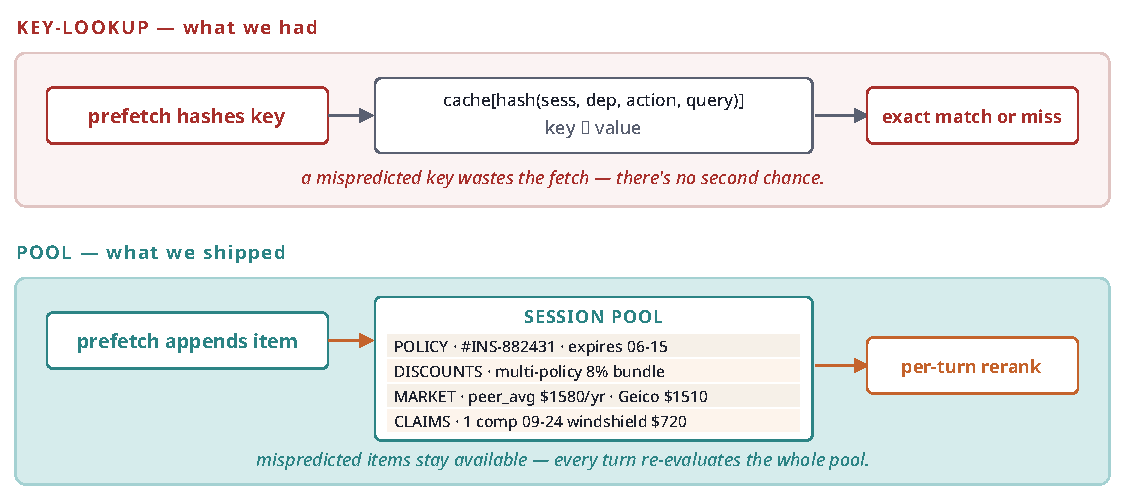
\includegraphics[width=0.80\linewidth]{figs/fig5_key_lookup_vs_pool.pdf}
\caption{Exact-key lookup (top) vs.\ the pool (bottom). Under key-lookup a mispredicted key wastes the fetch; under the pool, every fetched item stays available and the live agent curates per turn.}
\label{fig:keylookup-vs-pool}
\end{figure*}

When the needed data depends on what the user just said---RAG over policy documents or claims history---exact key prediction is unreliable: even good predictions are only approximately the live query. In an earlier measurement, 60\% of predicted RAG queries shared at least one retrieved document with the eventual live query---a strong but inexact signal that an exact-key cache discards as a miss. The pool keeps that signal: each fetched item is appended to the session pool, and curation matches against it per turn rather than against a predicted key (Figure~\ref{fig:keylookup-vs-pool}).

Two measurements on \emph{different denominators} bound the effect on car-insurance renewal; we report both explicitly rather than as one ratio.

\begin{center}\footnotesize\setlength{\tabcolsep}{4pt}
\begin{tabular}{lcc}
\toprule
metric (denominator) & exact-key & pool \\
\midrule
fetches consumed (of 144) & \textbf{11\%} & --- \\
turns w/ $\ge1$ item (of 68) & --- & \textbf{96\%}$^{\dagger}$ \\
\bottomrule
\end{tabular}
\end{center}
{\footnotesize $^{\dagger}$Measured under the earlier LLM-rerank curation, not the final cosine+dedup config.}

The two numbers count different things---fetches versus turns---so they are not a single hit-rate that ``rises from 11\% to 96\%.'' Together, though, they make the structural point: under exact-key lookup most speculative fetches are wasted (89\% never consumed), whereas under the pool a mispredicted fetch remains a curated candidate and the live agent still finds a usable item on almost every turn. This compares two variants of our own architecture; \S\ref{sec:limitations} specifies the published-baseline comparison (no-cache, naive per-turn RAG) that would isolate the speculative-population contribution on a like-for-like metric.

\subsection{Rerank latency, cross-SOP}
\label{sec:cross-sop}

Under the architecture as described---no LLM on the critical path, cosine\,+\,dedup curation, speculative-context prompt---$N{=}5$ per SOP:

\begin{table}[t]
\centering\small
\begin{tabular}{lcccc}
\toprule
SOP & Succ. & Mean & p95 & MCTS path \\
\midrule
car-insurance & 5/5 & 293\,ms & 490\,ms & 0/60 \\
medical & 5/5 & 304\,ms & 453\,ms & 0/60 \\
\midrule
\textbf{Agg.\ ($N{=}10$)} & \textbf{10/10} & \textbf{299} & \textbf{483} & \textbf{0/120} \\
\bottomrule
\end{tabular}
\caption{Per-SOP results under the locked configuration (no LLM on the critical path, cosine\,+\,dedup curation, speculative-context prompt). Latencies are rerank-step wall-clock. The ``MCTS path'' column is a design property, not a finding: with \texttt{tier3\_enabled=false} the router cannot elevate live MCTS, so this is 0 by construction. Source data: \texttt{table1\_sessions.jsonl} (exported from the run database).}
\label{tab:cross-sop}
\end{table}

110 rerank calls; p50 = 246\,ms, p99 = 848\,ms. The latency profile is near-identical across two SOPs of opposite shape ($\le 4\%$ spread in mean, $\le 8\%$ in p95). We disclose a selection caveat: the car-insurance cell is the 5 successful runs from a batch of 8 (two further runs terminated incompletely and one is reported below as a same-architecture 4/5 comparison); $N$ is small and this is a sampled slice, not an exhaustive batch. A third SOP (credit-card activation) is in the codebase; its earlier exclusion was an action-proposer issue in the SOP-graph gating, fixed in code but \emph{not yet re-benchmarked}---its inclusion is part of the breadth study in \S\ref{sec:limitations}.

\subsection{Pool composition}

Across the 97 fetches in the $N{=}10$ evaluation:

\begin{center}\small
\begin{tabular}{lcc}
\toprule
Source of fetch & Fetches & Share \\
\midrule
Empirical predictor (precedent traces) & 85 & 88\% \\
Blocking live fallback (a prefetch \emph{miss}) & 9 & 9\% \\
Background MCTS pondering & 3 & 3\% \\
\bottomrule
\end{tabular}
\end{center}

Only the empirical predictor and pondering are speculative \emph{predictions}; the 9 live-fallback fetches are misses served synchronously on the critical path (\S\ref{sec:arch}), reported here for completeness. The empirical predictor is load-bearing; the headline numbers do not depend on MCTS pondering, which is under-exercised by the test conditions: of the 213 pondering runs spawned across these sessions, 209 (98\%) were cancelled by the next user turn. (Pondering's mean duration of 7.4\,s is computed over a larger set of pondering runs than the 213 here; the autopilot's zero-pause turn cycle averages 6.0\,s.) Real calls have 2--5\,s inter-turn pauses, which would give pondering room to complete; \S\ref{sec:limitations} specifies the timing study that measures its contribution under realistic pauses.

Weighting these misses by latency gives a regret view (\S\ref{sec:related}): the 9 misses cost 34.7\,s of critical-path time in aggregate (mean 3.86\,s each, essentially equal to a pool hit's 3.86\,s, so the unweighted miss rate and the latency-weighted regret coincide here). Against the latency the pool removed, that is a realized latency-regret of 4.5\% versus a perfect-foresight oracle---the prefetcher captures 95.5\% of the available benefit (a converged point estimate, not a regret bound: the oracle is unbudgeted and our predictor is frozen).

\subsection{End-to-end latency, and what this work does not address}
\label{sec:e2e}

The rerank step is small, but it is not the whole turn. Over the Table~\ref{tab:cross-sop} sessions (\texttt{gpt-4o} live agent), mean end-to-end agent time per turn is \textbf{6.0\,s} (p50 5.3\,s, p95 10.9\,s), decomposed as: classify-and-propose 2.4\,s, response generation 1.8\,s, situation embedding 0.3\,s, and pool rerank 0.3\,s. The two live-agent LLM calls ($\approx$4.2\,s) dominate; the prefetch machinery this paper contributes adds only the $\sim$0.3\,s rerank.

What the architecture removes from the critical path is \emph{external-data} latency, not LLM latency. The six data dependencies per SOP carry 0.35--6.5\,s mocked fetch latencies; across our sessions the pool hides a mean of \textbf{22.5\,s} of such latency per conversation---data that, fetched synchronously, would otherwise land on the critical path. The $\sim$300\,ms rerank is the price of hiding that 22.5\,s.

A smaller live model does not shrink the 4.2\,s LLM floor. We re-ran the live agent on \texttt{gpt-4o-mini} ($N{=}10$, matched config): end-to-end turn time did \emph{not} improve (6.4\,s vs.\ 6.0\,s---the structured classify call was in fact 0.8\,s \emph{slower} on the smaller model, at identical output length), and session success fell from 10/10 to 4/10 (car-insurance collapsed to 0/5). For these hosted models, model tier did not predict per-request latency, and the weaker model's planning degraded enough to break task completion. Reducing the LLM floor therefore calls for streaming or speculative generation~\cite{lts2026,relays2s2026}---an orthogonal lever to the external-data problem we target.

%======================================================================
\section{Ablations}
\label{sec:ablations}
%======================================================================

\subsection{Why cosine\,+\,dedup, not an LLM rerank or a confidence gate}
\label{sec:abl-rerank}

The per-turn curation could be done by an LLM, by cosine ranking, or by cosine ranking gated by a confidence test. We compare them.

\textbf{An LLM rerank is unnecessary for relevance selection.} On a held-out run we computed, per turn, the LLM rerank's picks and the embedding ranking's top-8. 87\% of the LLM's picks were already in the embedding top-8; in 77\% of turns \emph{all} of the LLM's picks were. The LLM and embedding disagreed on rank within the top-$N$, not on which items belonged---except in one respect: the LLM avoided returning near-duplicate items, which a raw cosine ranking does not. The dedup pass (\S\ref{sec:rerank-design}) recovers exactly this. Cosine\,+\,dedup therefore matches the LLM's curation at no critical-path LLM cost. The table below reports the \emph{matched} comparison---LLM rerank and cosine\,+\,dedup measured under the same architecture and run set---rather than pairing a worst-case LLM run against a best-case cosine run; for reference, the locked cross-SOP configuration (Table~\ref{tab:cross-sop}) holds cosine\,+\,dedup at 299\,ms mean / 483\,ms p95.

\begin{center}\footnotesize\setlength{\tabcolsep}{4pt}
\begin{tabular}{lcc}
\toprule
rerank latency (matched) & LLM rerank & cosine+dedup \\
\midrule
mean & 1523\,ms & \textbf{378\,ms} \\
p95 & 2167\,ms & \textbf{940\,ms} \\
\bottomrule
\end{tabular}
\end{center}

\textbf{A confidence gate does not apply here.} A natural optimisation is to skip the LLM only when the embedding ranking is ``decisive'' (the $K$-th cosine clears an absolute floor and the gap to the $(K{+}1)$-th exceeds a margin). We set a 0.50 floor / 0.05 margin and, in our notes, expected 60--80\% adoption. Adoption was 0\%: pool items are conversationally homogeneous (same renewal, same customer), so cosines cluster in a tight low band rather than forming cliffs. The $K$-th cosine never exceeded 0.421 (Figure~\ref{fig:cosine}); the median $K$/$(K{+}1)$ gap was 0.013. The gate's premise---that some turns have a decisive embedding ranking---is false for this data, which is why we curate unconditionally rather than gate. (Reducing the LLM prompt's input tokens via a top-8 pre-filter is likewise ineffective: it cut input from $\sim$6--8K to $\sim$1.8K tokens but left p95 unchanged, because the fast model's cost is dominated by the call itself, not prompt length.)

\begin{figure}[t]
\centering
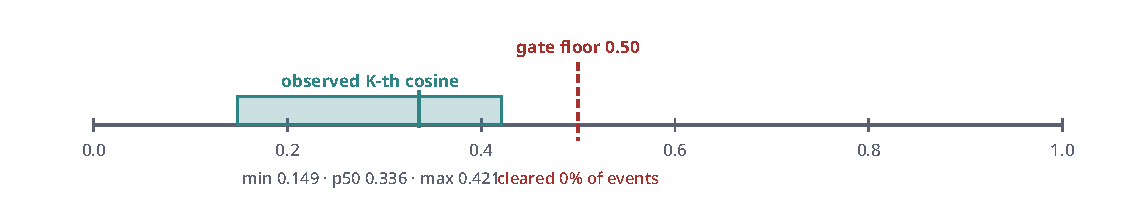
\includegraphics[width=\linewidth]{figs/fig6_cosine_distribution.pdf}
\caption{Live-message/pool-item cosine distribution over 44 gate-eligible turns. The observed $K$-th cosine (teal band, max 0.421) never reaches the 0.50 gate floor (dashed). Topically homogeneous pools do not produce the cliffs a confidence gate needs.}
\label{fig:cosine}
\end{figure}

\subsection{The speculative-context prompt is necessary}
\label{sec:abl-prompt}

Because the cosine rerank returns top-3 items unconditionally, it cannot decline on a turn where nothing in the pool is relevant---most visibly on conversation-closing turns, where the user winds down (``thanks, I'll get back to you'') and the top pool cosine falls to 0.10--0.18. The question is whether the live agent uses those low-relevance items. That depends on the prompt's framing. We hold the architecture fixed and vary only the label on the prefetched-context block:

\begin{center}\footnotesize
\setlength{\tabcolsep}{4pt}
\begin{tabular}{lccc}
\toprule
& Curated & Speculative & $\Delta$ \\
\midrule
Session success & 3/5 & \textbf{4/5}$^{*}$ & recov. \\
Mean rerank & 378\,ms & 320\,ms & --15\% \\
p95 rerank & 940\,ms & 429\,ms & --54\% \\
\bottomrule
\end{tabular}
\end{center}
{\footnotesize $^{*}$The remaining non-success was a turn-budget cap-hit on the turn the user agreed to renew---an action-proposer issue, not a curation failure.}

Under the ``curated, high-relevance'' framing the agent treats the items as authoritative and answers about discounts and coverage on turns where the user is leaving; under the speculative framing it ignores the misfits and closes the call. The latency difference is noise at this $N$; the success difference is the point. We considered a mechanical alternative---a cosine floor that returns zero items below a threshold---but it is a tuned heuristic stacked on a tuned heuristic, and it addresses the symptom (items present) rather than the cause (the prompt over-claims their reliability). The prompt fix is architecture-agnostic and requires no threshold.

\textbf{Observation, not yet a principle.} This is consistent with Shi et al.~\cite{shi2023}, who showed that instructing an LLM to ignore irrelevant context mitigates the distraction effect; our addition is the \emph{framing-mismatch} ablation in an asynchronous speculate/consume pipeline---that an over-confident ``curated'' label, versus an honest ``speculative'' one, is what tips the agent into over-using low-relevance items---and the closing-turn failure mode it exposes. Whether this hardens into a law for such pipelines (``the consumer's prompt should reflect the speculation's actual reliability'') is a hypothesis a single framing-pair on one SOP cannot establish; \S\ref{sec:limitations} specifies the multi-framing, multi-SOP study needed.

\subsection{What predicts retrieval, and why MCTS does not}
\label{sec:abl-predictor}

The supervisor's most expensive component is the background MCTS pondering of \S\ref{sec:pondering}. We measure whether it earns its cost for the only job it does on the pool---predicting what to prefetch. Retrieval prediction decomposes into three sub-tasks: (i)~\emph{which data source} (the next agent action, which names its dependencies); (ii)~\emph{structured parameters} (which customer, policy, vehicle)---not predicted at all, since they are session facts already on the blackboard once identity is established; and (iii)~the \emph{free-text query} a RAG dependency needs, which depends on the specific question the user will ask and is genuinely generative.

\textbf{Sub-task (i): which source.} We score next-action prediction against ground truth on 50 turn-transitions from logged sessions:

\begin{center}\footnotesize\setlength{\tabcolsep}{4pt}
\begin{tabular}{lccc}
\toprule
predictor & recall@3 & latency & tokens/turn \\
\midrule
\textbf{empirical} (count over traces) & \textbf{88\%} & $\sim$1\,ms & \textbf{0} \\
naive LLM (one call) & 38\% & 1.6\,s & $\sim$1.6K \\
MCTS pondering & 33\%$^{*}$ & 10.6\,s & $\sim$25.6K \\
\bottomrule
\end{tabular}
\end{center}
{\footnotesize $^{*}$modal next-action across rollouts (logged); pondering also has a 62\% cancellation rate.}

\noindent Counting wins decisively: predicting an agent's next move is a question about its \emph{habits}, which the empirical predictor memorizes from \texttt{precedent\_traces}; MCTS and the naive LLM reason about a \emph{hypothetical} future and do worse, at $10^3$--$10^4\times$ the token cost.

\textbf{Sub-task (iii): the generative query.} Only RAG dependencies need it. We render the query three ways---a structured stub (cohort/state/action only), a cheap single-LLM next-utterance prediction, and MCTS rollout text---and measure retrieved-document overlap against the query rendered from the \emph{actual} next user utterance, across corpora of increasing granularity:

\begin{center}\footnotesize\setlength{\tabcolsep}{5pt}
\begin{tabular}{lcccc}
\toprule
$\{$user\_text$\}$ source & coarse & fine & large & tok \\
& (25) & (44) & (63) & \\
\midrule
structured stub & 70\% & 48\% & 43\% & 0 \\
\textbf{cheap LLM} & 73\% & \textbf{62\%} & \textbf{54\%} & $\sim$300 \\
MCTS rollouts & 60\% & $\sim$60\% & $\sim$60\% & $\sim$25.6K \\
\bottomrule
\end{tabular}
\end{center}

\noindent The value of generative query prediction \emph{scales with corpus granularity}: when many documents share a cohort/state and differ only by the specific situation, the structured stub collapses (70$\to$43\%) while a single small-model utterance prediction holds an 11--14\,pp lead---matching MCTS at $\sim$85$\times$ lower cost. (The fine and large corpora are constructed stress-tests with realistic situation-variants, not production data.)

\textbf{Resolution.} Empirical counting for the action and structured parameters; one cheap LLM call for the generative query slot, gated on whether a RAG dependency is in the predicted horizon; MCTS for neither. This retires pondering from the retrieval path---a $\sim$99\% token reduction with \emph{higher} action accuracy---and aligns with concurrent findings that pattern-mined speculation from execution traces (PASTE~\cite{paste2026}) outperforms search-based lookahead for tool/data prefetch. We retain pondering in the architecture only as a cold-start option (when no traces have accumulated) and for its cached-decision payoff, both deferred to future evaluation.

%======================================================================
\section{Discussion}
%======================================================================

\textbf{When the pool reframe helps.} Whenever prefetch is driven by predictions that are \emph{approximately} right. The pool gives the system a second chance to use approximately-correct fetches; exact-key caching throws them away. The more the needed data depends on the live utterance (RAG, parameterised queries), the larger the gap.

\textbf{When cosine\,+\,dedup suffices.} When pool items live in the user's turn space, so embedding similarity tracks relevance (here, the 87\% LLM/embedding agreement). For highly heterogeneous pools spanning many domains, an LLM's discrimination may still add value beyond cosine ranking; the dedup pass is the minimal recovery of the LLM's contribution we observed.

\textbf{Scope of the prompt observation.} If the framing-mismatch result generalizes (\S\ref{sec:abl-prompt}), it would apply to any consumer reading from a speculatively-populated surface---blackboards, vector stores, search caches---as, in effect, the asynchronous-systems analogue of accurate API documentation: the interface should describe what it actually guarantees.

%======================================================================
\section{Limitations and the experiments that complete this work}
\label{sec:limitations}
%======================================================================

We are explicit that the present evaluation establishes the architecture's mechanics and internal consistency, not yet its standing against the field. The following experiments are planned to close that gap.

\begin{itemize}[leftmargin=*, itemsep=3pt]
\item \textbf{Statistical power.} Re-run every headline condition at $N\ge20$ per SOP with Wilson confidence intervals on rates and bootstrap intervals on latency percentiles. The present $N{=}5$ supports coarse confirmation only.
\item \textbf{Published baselines and a like-for-like metric.} The 11\%-consumed / 96\%-supplied pair compares two of our own variants on different denominators. The isolating comparison is against (a) no cache (live fetch), (b) naive per-turn RAG over a session vector store with no prefetch, and (c) an exact-key prefetch cache---all scored on one common metric (turns supplied a usable item), separating the value of \emph{speculative population} from the value of the pool data structure.
\item \textbf{A quality-linked metric.} Session success is coarse. We will add a per-turn data-grounding measure (did the reply correctly use available prefetched data on data-dependent questions?) and redefine effective hit rate as relevant-\emph{and}-used rather than merely returned.
\item \textbf{The prompt principle as a controlled study.} The speculative-context result is one framing pair on one SOP. A multi-framing grid (curated / neutral / speculative / speculative+examples) across both SOPs, ideally a second task, is needed to claim a general principle.
\item \textbf{Real users via a live-avatar harness.} We have built a testing harness in which a human speaks to a GPT-Realtime voice avatar steered by the supervisor under full SOP control. A human study (A/B with vs.\ without prefetch) converts ``simulator-only'' from a limitation into a validated result and is the single largest credibility upgrade available to us.
\item \textbf{MCTS pondering under realistic timing.} Re-run with injected 2--5\,s inter-turn pauses to measure pondering's completion rate and contribution; the present zero-pause condition cancels 98\% of pondering runs and so cannot speak to its value.
\item \textbf{From frozen exploitation to online learning.} Our predictor is pure exploitation of a frozen estimate and never explores (\S\ref{sec:related}). A contextual, budget-constrained bandit~\cite{licontextual2010,bwk2018} that explores at cold start and under distribution shift---evaluated by cumulative regret rather than the converged 4.5\% point estimate of \S\ref{sec:cross-sop}---is the principled generalisation of the predictor stack.
\item \textbf{Breadth and cost.} Include credit-card activation (the blocking action-proposer issue is fixed in code; re-evaluation pending) and a fourth domain; and report per-turn LLM-call and token cost for cosine\,+\,dedup vs.\ LLM rerank vs.\ naive RAG.
\end{itemize}

%======================================================================
\section{Conclusion}
%======================================================================

We presented a two-system architecture for SOP-constrained voice agents that moves external-data retrieval off the critical path: across our sessions the supervisor's speculative pool hides a mean of 22.5\,s of external-data latency per conversation while the curation step it adds costs only $\sim$300\,ms. We evaluated three components: a misprediction-tolerant pool cache (89\% of speculative fetches that an exact-key cache would waste remain usable, and the live agent finds a prefetched item on 96\% of turns); a cosine-plus-dedup rerank shown by a matched ablation to recover an LLM reranker's only value-add at a fraction of its latency; and a speculative-context prompt whose framing-mismatch ablation keeps the live agent from over-using low-relevance items. We are explicit about what this work does \emph{not} address: total turn time ($\sim$6\,s) is dominated by the live agent's own LLM calls, which a smaller model does not reduce (\S\ref{sec:e2e}); reducing that is the domain of streaming and speculative generation~\cite{lts2026,relays2s2026}, orthogonal to the data-latency problem we target. \S\ref{sec:limitations} lays out the controlled studies---larger $N$ with confidence intervals, published baselines on a common metric, a quality-linked metric, and a real-user avatar study---that bring the evaluation to full strength.

%======================================================================
\footnotesize
\begin{thebibliography}{9}
\setlength{\itemsep}{0pt}
\bibitem{voiceagentrag2026} Qiu, J., et al. \emph{VoiceAgentRAG: Solving the RAG Latency Bottleneck in Real-Time Voice Agents Using Dual-Agent Architectures}, 2026. arXiv:2603.02206.
\bibitem{lts2026} Zou, et al. \emph{LTS-VoiceAgent: A Listen-Think-Speak Framework for Efficient Streaming Voice Interaction via Semantic Triggering and Incremental Reasoning}, 2026. arXiv:2601.19952.
\bibitem{relays2s2026} Mai, L. \emph{RelayS2S: A Dual-Path Speculative Generation for Real-Time Dialogue}, 2026. arXiv:2603.23346.
\bibitem{predasr2023} Schwarz, A., He, D., Van Segbroeck, M., Hethnawi, M., and Rastrow, A. \emph{Personalized Predictive ASR for Latency Reduction in Voice Assistants}. Interspeech 2023. arXiv:2305.13794.
\bibitem{asyncmld2023} Yoshimaru, N., Okuma, M., Iio, T., and Hatano, K. \emph{AsyncMLD: Asynchronous Multi-LLM Framework for Dialogue Recommendation System}, 2023. arXiv:2312.13925.
\bibitem{chatsop2024} Li, Z., et al. \emph{ChatSOP: An SOP-Guided MCTS Planning Framework for Controllable LLM Dialogue Agents}, 2024. arXiv:2407.03884.
\bibitem{paste2026} Sui, Y., et al. \emph{Act While Thinking: Accelerating LLM Agents via Pattern-Aware Speculative Tool Execution}, 2026. arXiv:2603.18897.
\bibitem{specrag2024} Wang, Z., et al. \emph{Speculative RAG: Enhancing Retrieval Augmented Generation through Drafting}. ICLR 2025. arXiv:2407.08223.
\bibitem{gptcache2023} Bang, F. \emph{GPTCache: An Open-Source Semantic Cache for LLM Applications Enabling Faster Answers and Cost Savings}. Proc.\ 3rd Workshop for NLP Open-Source Software (NLP-OSS), 2023.
\bibitem{cag2024} Chan, B.~J., Chen, C.-T., Cheng, J.-H., and Huang, H.-H. \emph{Don't Do RAG: When Cache-Augmented Generation is All You Need for Knowledge Tasks}, 2024. arXiv:2412.15605.
\bibitem{plancache2025} Zhang, Q., Wornow, M., Wan, J., and Olukotun, K. \emph{Agentic Plan Caching: Test-Time Memory for Fast and Cost-Efficient LLM Agents}. NeurIPS 2025. arXiv:2506.14852.
\bibitem{mmr1998} Carbonell, J., and Goldstein, J. \emph{The Use of MMR, Diversity-Based Reranking for Reordering Documents and Producing Summaries}. SIGIR 1998.
\bibitem{shi2023} Shi, F., et al. \emph{Large Language Models Can Be Easily Distracted by Irrelevant Context}. ICML 2023. arXiv:2302.00093.
\bibitem{speculativedecoding2023} Leviathan, Y., Kalman, M., and Matias, Y. \emph{Fast Inference from Transformers via Speculative Decoding}, ICML 2023. arXiv:2211.17192.
\bibitem{lairobbins1985} Lai, T.~L., and Robbins, H. \emph{Asymptotically Efficient Adaptive Allocation Rules}. Advances in Applied Mathematics 6(1):4--22, 1985.
\bibitem{auer2002} Auer, P., Cesa-Bianchi, N., and Fischer, P. \emph{Finite-time Analysis of the Multiarmed Bandit Problem}. Machine Learning 47:235--256, 2002.
\bibitem{licontextual2010} Li, L., Chu, W., Langford, J., and Schapire, R.~E. \emph{A Contextual-Bandit Approach to Personalized News Article Recommendation}. WWW 2010. arXiv:1003.0146.
\bibitem{bwk2018} Badanidiyuru, A., Kleinberg, R., and Slivkins, A. \emph{Bandits with Knapsacks}. Journal of the ACM 65(3):13, 2018 (FOCS 2013). arXiv:1305.2545.
\bibitem{slivkins2019} Slivkins, A. \emph{Introduction to Multi-Armed Bandits}. Foundations and Trends in Machine Learning 12(1--2):1--286, 2019. arXiv:1904.07272.
\end{thebibliography}

\end{document}
